% 9 variables in here:
% h_1 = 10.0, h_2 = 10.0, h_3 = 10.0, ux_1 = 0.0, ux_2 = 0.0, ux_3 = 0.0, uy_1 = 0.0, uy_2 = 0.0, uy_3 = 0.0
\begin{figure}[ht]
\centering
  \subfloat[] {
    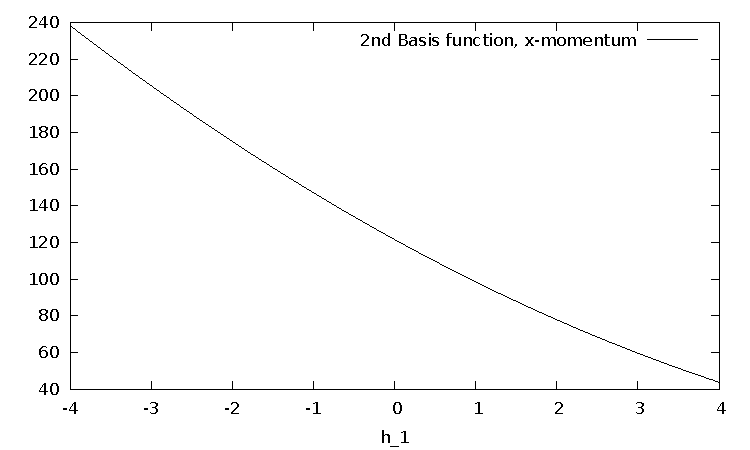
\includegraphics[scale=\zoomfactor]{{{20130208115342/y_10.0_10.0_0.0_0.0_0.0_0.0_0.0_0.0f2}}}
  }
  \subfloat[] {
    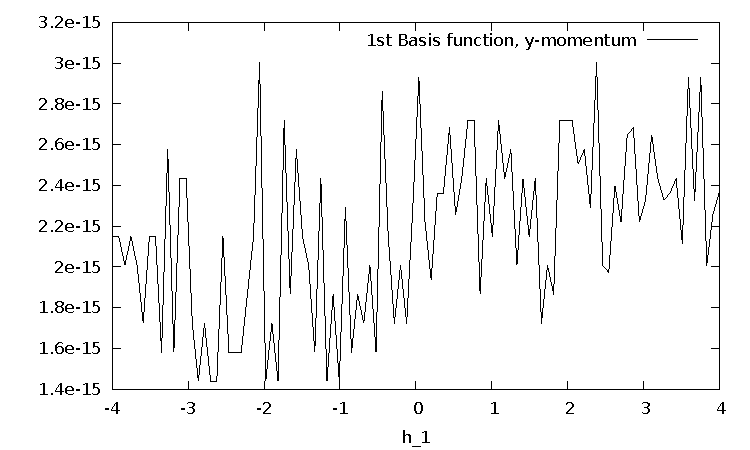
\includegraphics[scale=\zoomfactor]{{{20130208115342/y_10.0_10.0_0.0_0.0_0.0_0.0_0.0_0.0f1}}}
  }
  \subfloat[] {
    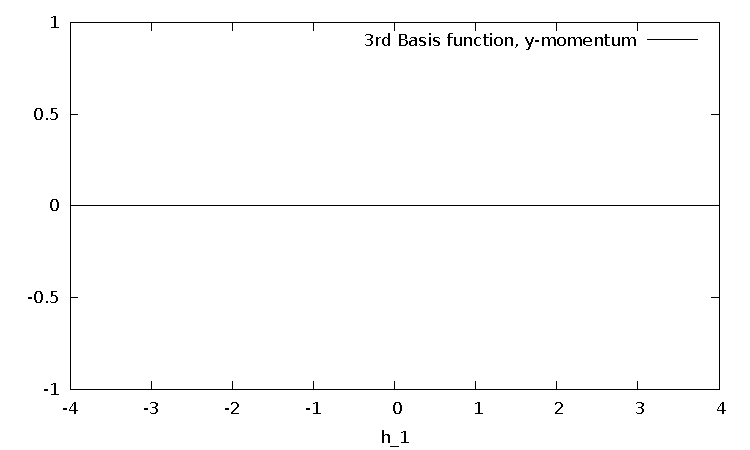
\includegraphics[scale=\zoomfactor]{{{20130208115342/y_10.0_10.0_0.0_0.0_0.0_0.0_0.0_0.0f5}}}
  }
  \subfloat[] {
    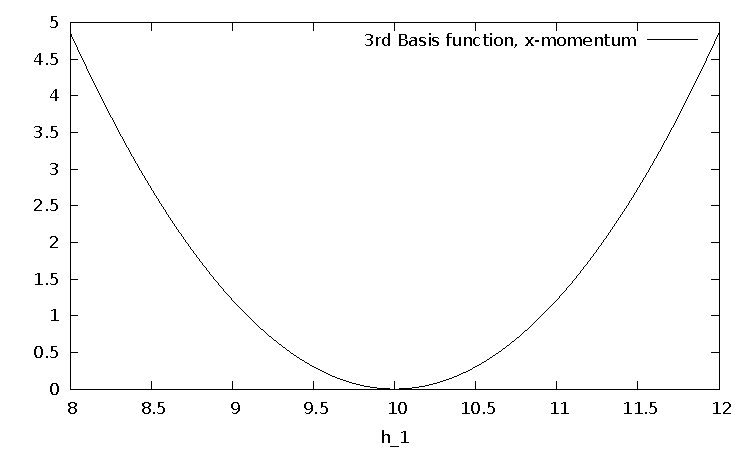
\includegraphics[scale=\zoomfactor]{{{20130208115342/y_10.0_10.0_0.0_0.0_0.0_0.0_0.0_0.0f4}}}
  }
  \subfloat[] {
    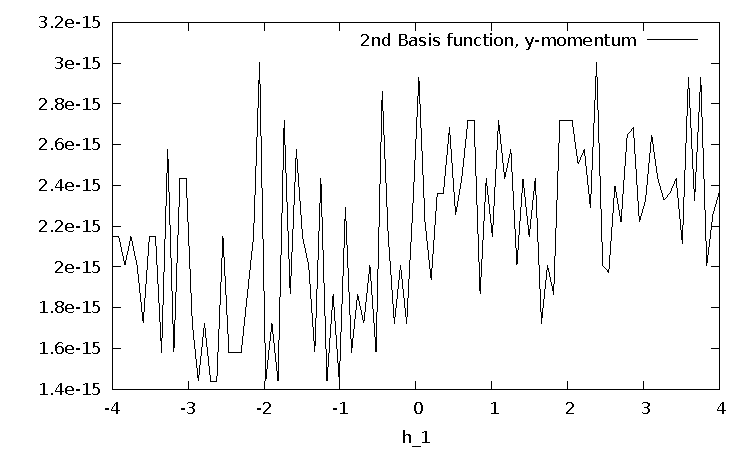
\includegraphics[scale=\zoomfactor]{{{20130208115342/y_10.0_10.0_0.0_0.0_0.0_0.0_0.0_0.0f3}}}
  }
  \subfloat[] {
    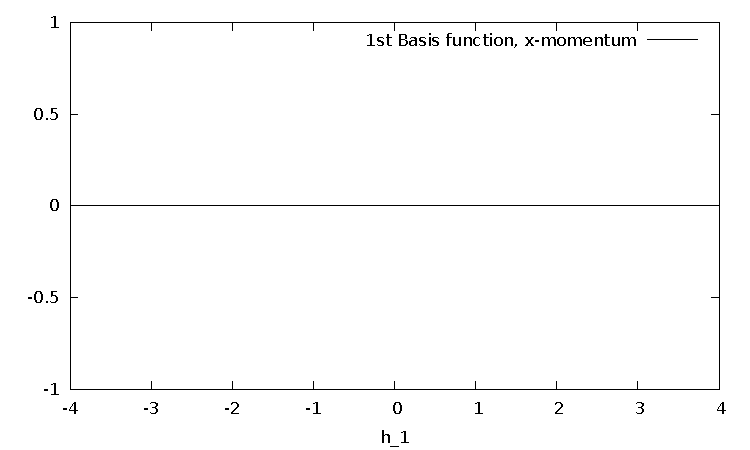
\includegraphics[scale=\zoomfactor]{{{20130208115342/y_10.0_10.0_0.0_0.0_0.0_0.0_0.0_0.0f0}}}
  }
\caption{}
\label{}
\end{figure}

%%% Local Variables:
%%% TeX-master: "../results.tex"
%%% End:
